\chapter{Analyse de l'existant}

\section{Les écoquartiers}

Un écoquartier est un quartier urbain conçu de manière à être respectueux de l'environnement et à promouvoir le développement durable. Il intègre des principes tels que la gestion efficace des ressources, la réduction des émissions de carbone, la promotion de la mobilité douce et l'utilisation d'énergies renouvelables.\\

Le fonctionnement d'un écoquartier repose sur plusieurs principes clés :
\begin{itemize}
\item \textbf{La gestion efficace des ressources :} un écoquartier vise à minimiser la consommation d'eau et d'énergie, ainsi que la production de déchets. Cela peut se faire en utilisant des technologies d'énergie renouvelable, en encourageant la réutilisation et le recyclage des matériaux, ou encore en favorisant les modes de transport doux comme le vélo ou les transports en commun.
\item \textbf{La conception urbaine durable :} un écoquartier est conçu pour encourager la cohésion sociale, en offrant des espaces verts et des lieux de rencontre pour les résidents. Il doit également être accessible à tous, notamment aux personnes à mobilité réduite.
\item \textbf{La participation des résidents :} les habitants de l'écoquartier sont encouragés à participer activement à la gestion du quartier, en prenant part aux décisions concernant l'aménagement et l'utilisation des espaces communs.
\item \textbf{La promotion de l'économie locale :} un écoquartier peut encourager l'installation d'entreprises locales et durables, favorisant ainsi l'emploi et l'économie locale.
\end{itemize}

\newpage

\section{L'entreprise et l'écoquartier}

\subsection{Présentation de LOCECO}

LOCECO est une entreprise engagée dans la gestion et la location d’appartements au sein d’un quartier écologique. Ils gèrent leurs appartements de manière responsable en minimisant la consommation d’énergie.\\

LOCECO souhaite promouvoir une démarche de consommation durable auprès de ces locataires. Pour encourager les résidents à trier leurs déchets et à recycler autant que possible, de multiples poubelles de tri sélectif sont disponibles dans les parties communes et des campagnes de sensibilisation pour expliquer aux résidents l'importance de cette pratique sont régulièrement organisées.

\subsection{Présentation d'une entreprise similaire : La SERS}

La SERS est une entreprise qui se spécialise dans l'aménagement de l'espace urbain et la construction d'écoquartiers dans le Grand Est de la France.\\

Elle vise à intégrer les principes du développement durable dans ses projets, notamment en ce qui concerne la mobilité, la gestion des déchets, l'empreinte environnementale et la mixité sociale. Par ailleurs, elle a défini un certains nombres de critères qui permet d’offrir un cadre de vie sain et sûr à ses habitants.\\

Un exemple concret de la part de cette entreprise est l'écoquartier "Les Prairies du Canal"

Le programme d’aménagement de ce quartier conçu par la SERS vise à offrir une cohérence environnementale avec une présence de la nature dans l’architecture. La hauteur est privilégiée pour libérer plus de 80\% d’emprise au sol. Ce site de 14 ha et de 1 300 logements à terme offre des qualités paysagères dont la principale est sans nul doute la présence du canal.

\begin{figure}[!h]
\begin{center}
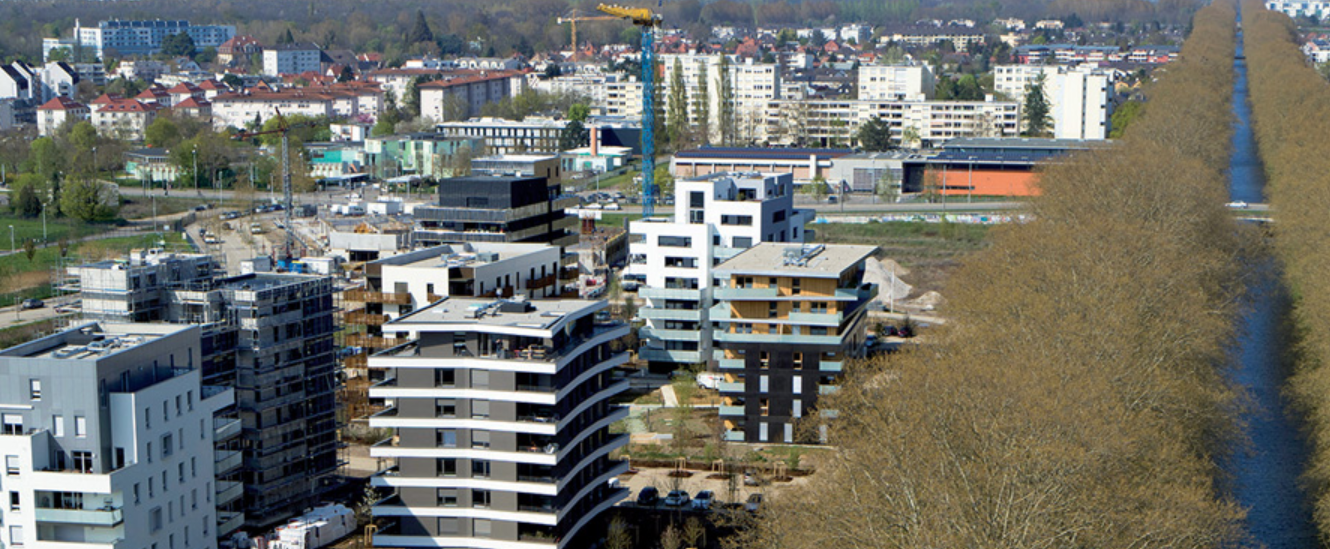
\includegraphics[width=15cm]{prairiescanal.png}
\end{center}
\caption{L'écoquartier Les Prairies du Canal en cours de construction}
\end{figure}





